\chapter{Espacio de clip y transformación de proyección}
En este paso los objetos son transformados del espacio de vista al espacio de clip utilizando la matriz \textbf{GL\_PROJECTION}. Esta matriz se utiliza para definir el frustum o tronco. Este frustum determina qué objetos o porciones de objetos serán recortados (\textit{clipped out}). También determina cómo se proyecta a la pantalla la escena 3D.

OpenGL proporciona dos funciones para la transformación de GL\_PROJECTION.

\begin{itemize}
\item{\textbf{glFrustum()}, para producir una proyección con perspectiva}
\item{\textbf{glOrtho()}, para producir una proyección ortográfica (paralela)}
\end{itemize}

Ambas funciones requieren 6 parámetros para especificar los 6 planos de corte; \textit{left}, \textit{right}, \textit{bottom}, \textit{top}, \textit{near} y \textit{far}.


También se puede utilizar \textbf{gluPerspective()}, que requiere de sólo 4 parámetros; el campo de vista vertical (FOV), la relación de aspecto de ancho a alto y las distancias a los planos de corte \textit{near} y \textit{far}. Es posible convertir la función gluPerspective() a glFrustum() con un código que será explicado en una sección posterior.

\section{Matriz de proyección (GL\_PROJECTION)}
Un monitor de ordenador es una superfície 2D. Una escena 3D renderizada por OpenGL tiene que ser proyectada a la pantalla del ordenador como una imagen 2D. La matriz GL\_PROJECTION es usada para esta transformación de proyección. Primero, la información de las coordenadas de vista es transformada a coordenadas de clip. Luego, estas coordenadas de clip son también transformadas a coorenadas normalizadas de dispositivo (NDC) dividiendo por el componente \textit{w} de las coordenadas de clip.

Por ello, tenemos que tener en cuenta que tanto el clipping (corte de frustum) como las transformaciones NDC están integradas en la matriz \textbf{GL\_PROJECTION}. Las siguientes secciones describen cómo construir la matriz de proyección utilizando 6 parámetros; \textit{left}, \textit{right}, \textit{bottom}, \textit{top}, \textit{near} y \textit{far}.

Nótese que el corte de frustum (clipping) se efectua en las coordenadas de clip, justo antes de dividir por $w_c$. Las coordenadas de clip, $x_c$, $y_c$ y $z_c$ se comprueban siendo comparadas con $w_c$. Si cualquiera de las coordenadas de clip es menor que $-w_c$, o más grande que $w_c$, entonces el vértice será descartado.
$ -w_c < x_c, y_c, z_c < wc $

Entonces, OpenGL rescunstruirá los filos del polígono donde ocurre el clipping.

\begin{figure} [h]
  \centering
  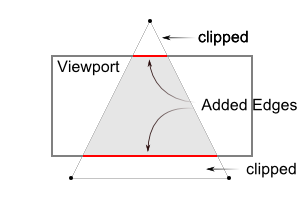
\includegraphics[width=0.3\textwidth]{gl_frustumclip}
  \caption{Un triangulo clipeado por el frustum}
\end{figure}

\section{Proyección de perspectiva}
En una proyección de perspectiva, un punto 3D en un en un frustum piramical truncado (coordenadas de vista) es mapeado a un cubo (NDC); el rango de la coordenada X desde [l, r] hasta [-1, 1], la coordenada Y desde [b, t] hasta [-1, 1] y la coordenada Z desde [n, f] hasta [-1, 1].

\begin{figure} [h]
  \centering
  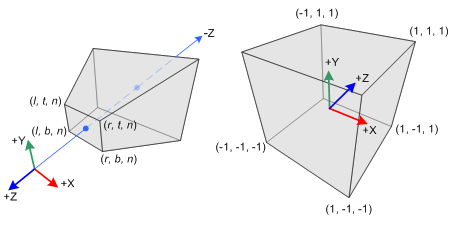
\includegraphics[width=0.6\textwidth]{gl_projectionmatrix01}
  \caption{Frustum de perspectiva y \textit{Normalized Device Coordinates} (NDC)}
\end{figure}


\newpage

Nótese que las coordenadas de vista están definidas por el sistema de coordenadas de la mano derecha, pero NDC utiliza el sistema de coordenadas de la mano izquierda. Por ello, la cámara en el origen está mirando a través del jee -Z en el espacio de vista, pero está mirando en el eje +Z en NDC. Puesto que \textbf{glFrustum()} sólo acepta valores positivos cómo distancias \textit{near} y \textit{far}, necesitamos negarlos durante la construcción de la matriz GL\_PROJECTION.

En OpenGL, un punto 3D en el espacio de vista es proyectado a el plano \textit{near} (plano de proyección). Los siguientes diagramas muestran como un punto $(x_v, y_v, z_v)$ en el espacio de vista está proyecatado a $(x_p, y_p, z_p)$ al plano \textit{near}.

\begin{figure} [h]
  \centering
  \captionsetup[subfigure]{justification=centering}
  \begin{subfigure}{0.3\textwidth} 
    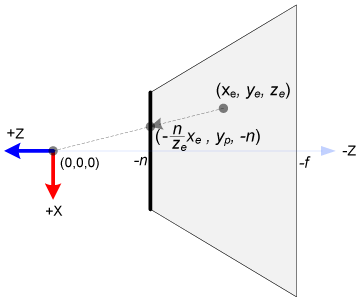
\includegraphics[width=\textwidth]{gl_projectionmatrix03} 
    \caption{Vista superior del Frustum}
  \end{subfigure}
  \begin{subfigure}{0.3\textwidth}
    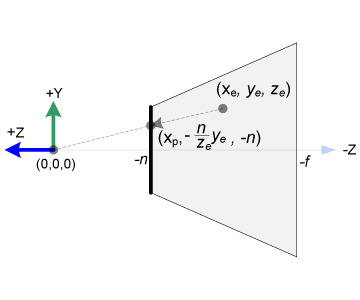
\includegraphics[width=\textwidth]{gl_projectionmatrix04} 
    \caption{Vista lateral del Frustum}
  \end{subfigure}
\end{figure}

Desde la vista superior del frustum, la coordenada X del espacio de vista, $x_v$ está mapeada a $x_p$, que es calculada utilizando la proporción de triangulos similares;
\begin{figure} [h]
  \centering
  \[
  \frac{x_p}{x_v} = \frac{-n}{z_v}
  x_p = \frac{-n \cdot x_v}{z_v} = \frac{n \cdot x_v}{-z_v}
  \]
\end{figure}

Desde la vista lateral del frustum, $y_p$ puede ser calculada con un método similar;

\begin{figure} [h]
  \centering
  \[ \frac{y_p}{y_v} = \frac{-n}{z_v}
  y_p = \frac{-n \cdot y_v}{z_v} = \frac{n \cdot y_v}{-z_v} \]
\end{figure}

\newpage
\newgeometry{top=25mm, bottom=27mm}
Nótese que tanto $x_p$ como $y_p$ dependen de $z_v$; son inversamente proporcionales a $-z_v$. En otras palabras, ambas están divididas por $-z_v$. Esta es la primera pista para la construcción de la matriz GL\_PROJECTION. Después de que las coordenadas sean transformadas multiplicando la matriz GL\_PROJECTION, las coordenadas siguien siendo coordenadas homogéneas. Se vuelven finalmente \textit{Normalized Device Coordinates} (NDC) cuando se dividen por el componente \textit{w} de las coordenadas de clip.

\begin{figure} [h]
  \centering
  \[
  \begin{pmatrix}
    x_{clip} \\ y_{clip} \\ z_{clip} \\ w_{clip}
  \end{pmatrix}
  =
  M_{projection} \cdot
  \begin{pmatrix}
    x_{vista} \\ y_{vista} \\ z_{vista} \\ w_{vista}
  \end{pmatrix} ,
  \begin{pmatrix}
    x_{ndc} \\ y_{ndc} \\ z_{ndc}
  \end{pmatrix}
  =
  \begin{pmatrix}
    x_{ndc}/w_{clip} \\ y_{ndc}/w_{clip} \\ z_{ndc}/w_{clip}
  \end{pmatrix}
  \]
\end{figure}


Entonces, podemos definir el componente \textit{w} de las coordenadas de clip como $-z_v$. Y la cuarta fila de la matriz GL\_PROJECTION se vuelve (0, 0, -1, 0).


\begin{figure} [h]
  \centering
  \[
  \begin{pmatrix}
    x_{clip} \\ y_{clip} \\ z_{clip} \\ w_{clip}
  \end{pmatrix}
  =
  M_{projection} \cdot
  \begin{pmatrix}
    \cdot && \cdot && \cdot && \cdot \\
    \cdot && \cdot && \cdot && \cdot \\
    \cdot && \cdot && \cdot && \cdot \\
        0 &&     0 &&    -1 &&     0
  \end{pmatrix} \cdot
  \begin{pmatrix}
    x_{vista} \\ y_{vista} \\ z_{vista} \\ w_{vista}
  \end{pmatrix}
  ,  \hspace*{0.5cm} \therefore w_c = -z_v
  \]
\end{figure}


Después, mapeamos $x_p$ y $y_p$ a $x_n$ y $y_n$ de NDC con una relación linear; \([l, r] \implies [-1, 1] \) y \([b, t] \implies [-1, 1]\).



\begin{figure} [h!]
  \centering
\begin{minipage}{0.25\textwidth}
  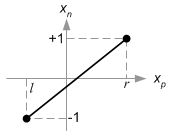
\includegraphics[width=\textwidth]{gl_projectionmatrix05}
  \caption{Mapeado de $x_p$ a $x_n$}
\end{minipage} \hspace*{2cm}
\begin{minipage}{0.3\textwidth}
\begin{flalign*}
   x_n &= \frac{1-(-1)}{r-l} \cdot x_p + \beta  \\
   1   &=  \frac{2r}{r - l} + \beta \hspace*{0.5cm} \textcolor{gray}{(sustituir (r,1) en (x_p, x_n))} \\
 \beta &= 1 - \frac{2r}{r-l} = \frac{r-l}{r-l} - \frac{2r}{r-l}\\
       &=\frac{r - l - 2r}{r - l} = \frac{-r -l}{r-l} = - \frac{r+l}{r-l} \\
   \therefore x_n &= \frac{2x_p}{r-l}-\frac{r+l}{r-l} \\
\end{flalign*}
\end{minipage}

\end{figure}

\begin{figure} [h!]
  \centering
\begin{minipage}{0.25\textwidth}
  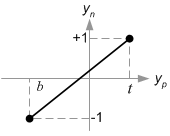
\includegraphics[width=\textwidth]{gl_projectionmatrix06}
  \caption{Mapeado de $y_p$ a $y_n$}
\end{minipage} \hspace*{2cm}
\begin{minipage}{0.3\textwidth}
\begin{flalign*}
   y_n &= \frac{1-(-1)}{t-b} \cdot y_p + \beta \\
     1 &=  \frac{2t}{t - b} + \beta \hspace*{0.5cm} \textcolor{gray}{(sustituir (t,1) en (y_p, y_n))} \\ 
 \beta &= 1 - \frac{2t}{t-b} = \frac{t-b}{t-b} - \frac{2t}{t-b}\\
       &=   \frac{t - b - 2t}{t - b} = \frac{-t -b}{t-b} = - \frac{t+b}{t-b} \\
\therefore y_n &= \frac{2y_p}{t-b}-\frac{t+b}{t-b} \\
\end{flalign*}
\end{minipage}

\end{figure}
\restoregeometry

Ahora, sustituimos $x_p$ y $y_p$ a esas ecuaciones.

\begin{figure} [h]
  \centering
  \begin{minipage}{0.45\textwidth}
    \begin{flalign*}
      x_n &= \frac{2x_p}{r-l} - \frac{r+l}{r-l} \hspace*{0.5cm} \textcolor{gray}{(x_p = \frac{nx_e}{-z_e})}\\
          &= \frac{2 \cdot \frac{n \cdot x_e }{-z_e}}{r-l} - \frac{r+l}{r-l}\\
          &= \frac{2n \cdot x_e}{(r-l)(-z_e)} - \frac{r+l}{r-l}\\
          &= \frac{\frac{2n}{r-l} \cdot x_e}{-z_e} - \frac{r+l}{r-l}\\
          &= \frac{\frac{2n}{r-l} \cdot x_e}{-z_e} + \frac{\frac{r+l}{r-l}\cdot z_e}{-z_e}\\
          &= \Big( \underbrace{\frac{2n}{r-l}\cdot x_e + \frac{r+l}{r-l}\cdot z_e}_{{x_c}} \Big) \Big/ -z_e
    \end{flalign*}
  \end{minipage}
  \begin{minipage}{0.45\textwidth}
    \begin{flalign*}
      y_n &= \frac{2y_p}{t-b} - \frac{t+b}{t-b} \hspace*{0.5cm} \textcolor{gray}{(y_p = \frac{ny_e}{-z_e})}\\
          &= \frac{2 \cdot \frac{n \cdot y_e }{-z_e}}{t-b} - \frac{t+b}{t-b}\\
          &= \frac{2n \cdot y_e}{(t-b)(-z_e)} - \frac{t+b}{t-b}\\
          &= \frac{\frac{2n}{t-b} \cdot y_e}{-z_e} - \frac{t+b}{t-b}\\
          &= \frac{\frac{2n}{t-b} \cdot y_e}{-z_e} + \frac{\frac{t+b}{t-b}\cdot z_e}{-z_e}\\
          &= \Big( \underbrace{\frac{2n}{t-b}\cdot y_e + \frac{t+b}{t-b}\cdot z_e}_{y_c} \Big) \Big/ -z_e
    \end{flalign*}
  \end{minipage}
\end{figure}

Nótese que hacemos que ambos términos sean divisibles por $-z_e$ para la división de perspectiva ($x_c/w_c$, $y_c/w_c$). Y ya establecimos que $w_c = -z_e$ anteriormente, y que los términos dentro del paréntesis se vuelven las coordenadas $x_c$ y $y_c$ de las coordenadas de clip.


De estas dos ecuaciones, podemos encontrar la primera y segunda fila de la matriz GL\_PROJECTION.

\begin{figure}[h]
  \[
  \begin{pmatrix}
    x_{clip} \\ y_{clip} \\ z_{clip} \\ w_{clip}
  \end{pmatrix}
  =
  \begin{pmatrix}
    \frac{2n}{r-l} &&              0 && \frac{r+l}{r-l} &&     0 \\
                 0 && \frac{2n}{t-b} && \frac{t+b}{t-b} &&     0 \\
             \cdot &&          \cdot &&           \cdot && \cdot \\
                 0 &&              0 &&              -1 &&     0
  \end{pmatrix}
  \cdot
  \begin{pmatrix}
    x_{vista} \\ y_{vista} \\ z_{vista} \\ w_{vista}
  \end{pmatrix}
  \]
\end{figure}

\newpage

Ahora sólo queda la tercera fila de la matriz GL\_PROJECTION por resolver. Encontrar $z_n$ es un poco más diferente de los demás porque en $z_{vista}$ en el espacio de vista está siempre proyectado hacia $-n$ en el plano \textit{near}. Pero ahora necesitamos un valor \textit{z} único para el clipping y la prueba de profundidad. Además, deberíamos de ser capaces de desproyectar (transformación inversa). Puesto que sabemos que \textit{z} no depende del valor \textit{x} o \textit{y}, tomamos prestado el componente \textit{w} para encontrar la relación entre $z_{ndc}$ y $z_{vista}$. Entonces, podemos especificar la tercera fila de la matriz GL\_PROJECTION de la siguiente forma.

\begin{figure}[h]
  \[
  \begin{pmatrix}
    x_{clip} \\ y_{clip} \\ z_{clip} \\ w_{clip}
  \end{pmatrix}
  =
  \begin{pmatrix}
    \frac{2n}{r-l} &&              0 && \frac{r+l}{r-l} &&     0 \\
                 0 && \frac{2n}{t-b} && \frac{t+b}{t-b} &&     0 \\
                 0 &&              0 &&               A &&     B \\
                 0 &&              0 &&              -1 &&     0
  \end{pmatrix}
  \cdot
  \begin{pmatrix}
    x_{vista} \\ y_{vista} \\ z_{vista} \\ w_{vista}
  \end{pmatrix}
  ,\hspace*{0.5cm} z_{ndc} = \frac{z_{clip}}{w_{clip}} = \frac{Az_{vista} + Bw_{vista}}{-z_e}
  \]
\end{figure}

En el espacio de vista, $w_{vista} = 1$. Por lo tanto, la ecuación se vuelve;

\begin{equation*}
  z_{ndc} = \frac{Az_{vista} + B}{-z_e} 
\end{equation*}
  
Para encontrar los coeficientes \textit{A} y \textit{B} usamos la relación $(Z_{vista}, Z_{ndc})$; $(-n, -1)$ y $(-f, 1)$, y las ponemos en la ecuación de arriba.

\begin{flalign*}
  \begin{cases}
    \frac{-An+B}{n} = -1 \\
    \frac{-Af+B}{f} = 1  \\
  \end{cases}
  \to
  \begin{cases}
    -An+B = -n \hspace*{1cm} \textcolor{gray}{(1)} \\
    -Af+B = f \hspace*{1.28cm} \textcolor{gray}{(2)}  \\
  \end{cases}  
\end{flalign*}

Para resolver las ecuaciones para \textit{A} y \textit{B}, se reescribe la ecuación (1) para \textit{B};
\begin{flalign*}
  B=An-n
\end{flalign*}

Se sustituye B en la ecuación (2) por la ecuación anterior y se aisla A;
\begin{gather*}
  -Af + (An - n) = f \\
  -(f-n)A = f+n \\ 
  A = - \frac{f+n}{f-n}
\end{gather*}

Se sustituye \textit{A} en la ecuación (1) para encontrar \textit{B};
\[
  \Big(\frac{f+n}{f-n}\Big)n + B = -n 
\]
\begin{flalign*}
  B &= -n - \Big(\frac{f+n}{f-n}\Big)n = - \Big( 1 + \frac{f+n}{f-n}\Big)n = - \Big(\frac{f-n+f+n}{f-n}\Big)n \\
  &= - \frac{2fn}{f-n}
\end{flalign*}


Se han hallado \textit{A} y \textit{B}. Por lo tanto, la relación entre $z_{vista}$ y $z_{ndc}$ se vuelve;

\[
z_n = \frac{-\frac{f+n}{f-n}z_v - \frac{2fn}{f-n}}{-z_v} \hspace*{1cm} \textcolor{gray}{(3)}
\]

Finalmente, se han encontrado todas las entradas de la matriz GL\_PROJECTION. La matriz de proyección completa es;

\begin{figure} [h]
  \[
  \begin{pmatrix}
    \frac{2n}{r-l} &&              0 &&   \frac{r+l}{r-l} &&                0 \\
                 0 && \frac{2n}{t-b} &&   \frac{t+b}{t-b} &&                0 \\
                 0 &&              0 && \frac{-(f+n)}{f-n} && \frac{-2fn}{f-n} \\
                 0 &&              0 &&                -1 &&                0
  \end{pmatrix}
  \]
  \caption{Matriz de proyección de perspectiva de OpenGL}
\end{figure}

Esta matriz de proyección es para un frustum general. Si el volumen de vista es simétrico, es decir, $r = -l$ y $t = -b$, entonces puede ser simplificada como;

\begin{equation*}
  \begin{cases}
    r+l = 0\\
    r-l = 2r \hspace*{0.2cm} \textcolor{gray}{(anchura)} \\
  \end{cases}
  \hspace*{0.3cm} , \hspace*{0.3cm}
  \begin{cases}
    t+b=0 \\
    t-b=2t \hspace*{0.2cm} \textcolor{gray}{(altura)} \\
  \end{cases}
\end{equation*}

\begin{figure} [h]
  \[
  \begin{pmatrix}
    \frac{n}{r} &&           0 &&                  0 &&                0 \\
              0 && \frac{n}{t} &&                  0 &&                0 \\
              0 &&           0 && \frac{-(f+n)}{f-n} && \frac{-2fn}{f-n} \\
              0 &&           0 &&                 -1 &&                0
  \end{pmatrix}
  \]
\end{figure}


\newpage

%% Aún falta una parte más que tampoco consideraba muy importante.

\section{Proyección ortográfica}
Construir la matriz GL\_PROJECTION para la proyección ortográfica es mucho más simple que para la proyección de perspectiva.

\begin{figure} [h]
  \centering
  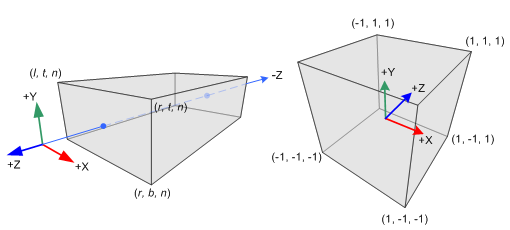
\includegraphics[width=0.6\textwidth]{gl_projectionmatrix02}
  \end{figure}

Los componentes $x_{vista}$, $y_{vista}$ y $z_{vista}$ en el espacio de vista son mapeados linearmente a NDC. Sólo es necesario escalar el volumen rectangular al cubo, y luego moverlo al origen. Ahora se econtrarán los elementos de GL\_PROJECTION utilizando relaciones lineares.

\begin{figure} [h!]
  \centering
\begin{minipage}{0.25\textwidth}
  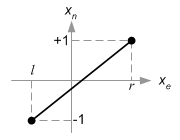
\includegraphics[width=\textwidth]{gl_projectionmatrix08}
  \caption{Mapeado de $x_v$ a $x_n$}
\end{minipage} \hspace*{2cm}
\begin{minipage}{0.3\textwidth}
\begin{flalign*}
   x_n &= \frac{1-(-1)}{r-l} \cdot x_v + \beta  \\
   1   &=  \frac{2r}{r - l} + \beta \hspace*{0.5cm} \textcolor{gray}{(sustituir (r,1) en (x_v, x_n))} \\
 \beta &= 1 - \frac{2r}{r-l} = - \frac{r+l}{r-l}\\
   \therefore x_n &= \frac{2}{r-l}\cdot x_v-\frac{r+l}{r-l} \\
\end{flalign*}
\end{minipage}
\end{figure}

\begin{figure} [h!]
  \centering
\begin{minipage}{0.25\textwidth}
  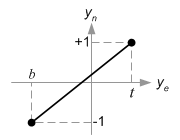
\includegraphics[width=\textwidth]{gl_projectionmatrix09}
  \caption{Mapeado de $y_v$ a $y_n$}
\end{minipage} \hspace*{2cm}
\begin{minipage}{0.3\textwidth}
\begin{flalign*}
   x_n &= \frac{1-(-1)}{t-b} \cdot x_v + \beta  \\
   1   &=  \frac{2t}{t - b} + \beta \hspace*{0.5cm} \textcolor{gray}{(sustituir (t,1) en (y_v, y_n))} \\
 \beta &= 1 - \frac{2t}{t-b} = - \frac{t+b}{t-b}\\
   \therefore y_n &= \frac{2}{t-b}\cdot y_v-\frac{t+b}{t-b} \\
\end{flalign*}
\end{minipage}
\end{figure}

\begin{figure} [h!]
  \centering
\begin{minipage}{0.25\textwidth}
  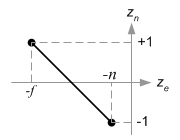
\includegraphics[width=\textwidth]{gl_projectionmatrix10}
  \caption{Mapeado de $z_v$ a $z_n$}
\end{minipage} \hspace*{2cm}
\begin{minipage}{0.3\textwidth}
\begin{flalign*}
   z_n &= \frac{1-(-1)}{-f-(-n)} \cdot z_v + \beta  \\
   1   &=  \frac{2f}{f - n} + \beta \hspace*{0.5cm} \textcolor{gray}{(sustituir (-f,1) en (z_v, z_n))} \\
 \beta &= 1 - \frac{2f}{f-n} = - \frac{f+n}{f-n}\\
   \therefore z_n &= \frac{-2}{f-n}\cdot z_v-\frac{f+n}{f-n} \\
\end{flalign*}
\end{minipage}
\end{figure}

\newpage

Puesto que el componente \textit{w} no es necesario para la proyección ortográfica, la cuarta fila de la matriz GL\_PROJECTION permanece como $(0,0,0,1)$. Por lo tanto, la matriz GL\_PROJECTION completa para la proyección otrográfica es;

\begin{figure} [h!]
  \[
  \begin{pmatrix}
    \frac{2}{r-l} &&             0 && - \frac{r+l}{r-l} &&                0 \\
                0 && \frac{2}{t-b} && - \frac{t+b}{t-b} &&                0 \\
                0 &&             0 &&    \frac{-2}{f-n} && -\frac{f+n}{f-n} \\
                0 &&             0 &&                  0 &&                1
  \end{pmatrix}
  \]
  \caption{Matriz de proyección otrográfica de OpenGL}
\end{figure}

Puede ser más simplificada si el volumen de vista es simétrico, $r=-l$ y $t=-b$.
\begin{figure} [h!]
\begin{equation*} 
  \begin{cases}
    r+l = 0\\
    r-l = 2r \hspace*{0.2cm} \textcolor{gray}{(anchura)} \\
  \end{cases}
  \hspace*{0.3cm} , \hspace*{0.3cm}
  \begin{cases}
    t+b=0 \\
    t-b=2t \hspace*{0.2cm} \textcolor{gray}{(altura)} \\
  \end{cases}
\end{equation*}
\end{figure}

\begin{figure} [h!]
  \[
  \begin{pmatrix}
    \frac{1}{r} &&           0 &&                 0 &&                0 \\
              0 && \frac{1}{t} &&                 0 &&                0 \\ 
              0 &&           0 &&    \frac{-2}{f-n} && -\frac{f+n}{f-n} \\ 
              0 &&           0 &&                 0 &&                1
  \end{pmatrix}
  \]
\end{figure}
